\documentclass{article}
\usepackage{122}

\usepackage{wrapfig}
\usepackage{tikz}
\usetikzlibrary{calc, positioning, shapes.gates.logic.US}
\usepackage{tkz-berge}

\usepackage{environ}
\NewEnviron{centerframebox}{\begin{center}\fbox{\parbox{0.92\textwidth}{\BODY}}\end{center}}

\newcommand{\NP}{\ensuremath{\mathsf{NP}}}
\newcommand{\NC}{\ensuremath{\mathsf{NC}^1}}
\newcommand{\PSPACE}{\ensuremath{\mathsf{PSPACE}}}
\renewcommand{\P}{\ensuremath{\mathsf{P}}}

\title{Теория сложности вычислений \\ Домашнее задание №6, №7 и №8}
\author{\AA{AAAAA AAAAAAA}{4} \\ \AA{AAAAAA}{13}}

\begin{document}
  \maketitle

  \setcounter{section}{5}
  \section{Домашнее задание №6}
  \setcounter{subsection}{8}
  \subsection{Define the function $\mathrm{majority}_n: \{0,\, 1\}^n \to \{0,\, 1\}$ as}
  $$\mathrm{majority}_n(x_1,\dots,x_n) = \begin{cases}
    0 & \sum x_i < n/2;\\
    1 & \sum x_i \geq n/2.\\
  \end{cases}$$
  \subsubsection{Show that $\mathrm{majority}_n$ can be computed with $O(n^2)$ size circuits.}
  Для этого решения мы можем просто отсортировать входное слово обычным пузырьком, и потом посмотреть на средний бит.
  Сортировку, то есть swap, дух битов мы можем построить просто из одного AND и одного OR gate-а:
  максимальный бит будет $\max(a,\, b) = a \land b$, а минимальный $\min(a,\, b) = a \lor b$.
  И для сортировки пузырьком нам понадобиться $n^2$ таких swap gate-ов.

  \subsubsection{Show that $\mathrm{majority}_n$ can be computed with $O(n\log n)$ size circuits.}
  Здесь мы можем построить $n$ бинарных счётчиков, каждый размером $\log n$, и так посчитать количество $1$-чек во входном слове.
  Такие счётчики можно собрать либо из full adder-ов, где просто одно из числе всегда нулевое, за исключением младшего бита, либо мы можем придумать специализированную схему для инкриминирования числа из одного XOR-а и одного AND-а (тоесть half adder) на каждый бит.
  Потом можно будет вычесть, то есть добавить two's complement, из результата константный $n/2$.
  И в качестве ответа мы сможем использовать последний бит счётчика.

  \begin{center}
    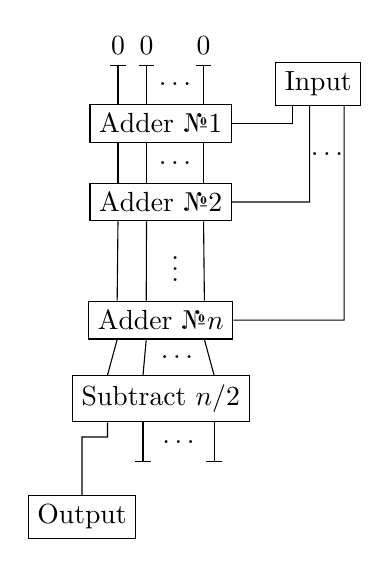
\begin{tikzpicture}
      \node[draw] (a1) at (0,0) {Adder №1};
      \node[draw] (a2) at (0,-1) {Adder №2};
      \node[draw] (a3) at (0,-2.5) {Adder №$n$};
      \node[draw] (a4) at (0,-3.5) {Subtract $n/2$};
      \node[draw] (i) at (2,.5) {Input};
      \node[draw] (o) at (-1,-5) {Output};

      \draw[-|] ($(a1.north west)!.2!(a1.north east)$) -- ++(0,.5) node[above] {$0$};
      \draw[-|] ($(a1.north west)!.4!(a1.north east)$) -- ++(0,.5) node[above] {$0$};
      \path ($(a1.north west)!.6!(a1.north east)$) -- node {$\dots$} ++(0,.5);
      \draw[-|] ($(a1.north west)!.8!(a1.north east)$) -- ++(0,.5) node[above] {$0$};

      \draw ($(a1.south west)!.2!(a1.south east)$) -- ($(a2.north west)!.2!(a2.north east)$);
      \draw ($(a1.south west)!.4!(a1.south east)$) -- ($(a2.north west)!.4!(a2.north east)$);
      \path ($(a1.south west)!.6!(a1.south east)$) -- node {$\dots$} ($(a2.north west)!.6!(a2.north east)$);
      \draw ($(a1.south west)!.8!(a1.south east)$) -- ($(a2.north west)!.8!(a2.north east)$);

      \draw ($(a2.south west)!.2!(a2.south east)$) -- ($(a3.north west)!.2!(a3.north east)$);
      \draw ($(a2.south west)!.4!(a2.south east)$) -- ($(a3.north west)!.4!(a3.north east)$);
      \path ($(a2.south west)!.6!(a2.south east)$) -- node {$\vdots$} ($(a3.north west)!.6!(a3.north east)$);
      \draw ($(a2.south west)!.8!(a2.south east)$) -- ($(a3.north west)!.8!(a3.north east)$);

      \draw ($(a3.south west)!.2!(a3.south east)$) -- ($(a4.north west)!.2!(a4.north east)$);
      \draw ($(a3.south west)!.4!(a3.south east)$) -- ($(a4.north west)!.4!(a4.north east)$);
      \path ($(a3.south west)!.6!(a3.south east)$) -- node {$\dots$} ($(a4.north west)!.6!(a4.north east)$);
      \draw ($(a3.south west)!.8!(a3.south east)$) -- ($(a4.north west)!.8!(a4.north east)$);

      \draw ($(a4.south west)!.2!(a4.south east)$) -- ($(a4.south west)!.2!(a4.south east|-o.north)$) -- ($(o.north|-a4.south west)!.2!(o.north)$) -- (o.north);
      \draw[-|] ($(a4.south west)!.4!(a4.south east)$) -- ++(0,-.5);
      \path ($(a4.south west)!.6!(a4.south east)$) -- node {$\dots$} ++(0,-.5);
      \draw[-|] ($(a4.south west)!.8!(a4.south east)$) -- ++(0,-.5);

      \draw ($(i.south west)!.2!(i.south east)$) -- ($(i.south west|-a1.east)!.2!(i.south east|-a1.east)$) -- (a1.east);
      \draw ($(i.south west)!.4!(i.south east)$) -- ($(i.south west|-a2.east)!.4!(i.south east|-a2.east)$) -- (a2.east);
      \path ($(i.south west)!.6!(i.south east)$) -- node {$\dots$} ($(i.south west|-a2.east)!.6!(i.south east|-a2.east)$);
      \draw ($(i.south west)!.8!(i.south east)$) -- ($(i.south west|-a3.east)!.8!(i.south east|-a3.east)$) -- (a3.east);
    \end{tikzpicture}
  \end{center}

  \subsection{The function $\mathrm{IP}(x,\, y)$ computes the inner product of vectors $x,\, y \in \{0,\, 1\}^n$ over the field $\mathbb{F}_2$. Show that $\mathrm{IP} \in \NC$.}
  Inner product in $\mathbb{F}_2$ это просто скалярное произведение $\ds x \cdot y = \sum_{i=0} x_i \cdot y_i$, и если считать $x$ и $y$ двоичными числами, то можно определить это скалярное произведение как количество единичек (по модулю $\mod 2$) в результате побитного AND.
  Класс \NC, в отличие от других нам знакомых классов, определяется не через машины Тьюринга, а через либо параллельные машины произвольного доступа (PRAM), либо через circuits ограниченной глубины.

  \begin{center}
    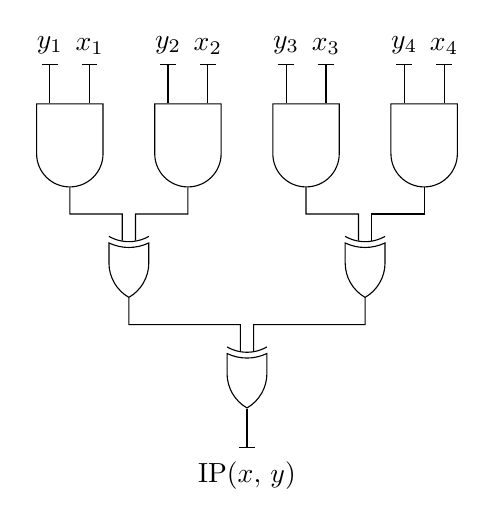
\begin{tikzpicture}
      \foreach \i in {1,2,3,4} {
        \node[and gate US, draw, rotate=-90, logic gate inputs=nnnn] (And\i) at (\i*1.5,0) {};
        \draw[-|] (And\i.input 1) -- ++(0,.5) node[above] {$x_\i$};
        \draw[-|] (And\i.input 4) -- ++(0,.5) node[above] {$y_\i$};
      }

      \path ($(And1.output)!0.5!(And2.output)$) -- node[xor gate US, draw, rotate=-90, logic gate inputs=nn] (Xor1) {} ++(0,-2);
      \draw (Xor1.input 2) -- ($(Xor1.input 2|-And1.output)!0.5!(Xor1.input 2)$) -- ($(And1.output|-Xor1.input 2)!0.5!(And1.output)$) -- (And1.output);
      \draw (Xor1.input 1) -- ($(Xor1.input 1|-And2.output)!0.5!(Xor1.input 1)$) -- ($(And2.output|-Xor1.input 1)!0.5!(And2.output)$) -- (And2.output);

      \path ($(And3.output)!0.5!(And4.output)$) -- node[xor gate US, draw, rotate=-90, logic gate inputs=nn] (Xor2) {} ++(0,-2);
      \draw (Xor2.input 2) -- ($(Xor2.input 2|-And3.output)!0.5!(Xor2.input 2)$) -- ($(And3.output|-Xor2.input 2)!0.5!(And3.output)$) -- (And3.output);
      \draw (Xor2.input 1) -- ($(Xor2.input 1|-And4.output)!0.5!(Xor2.input 1)$) -- ($(And4.output|-Xor2.input 1)!0.5!(And4.output)$) -- (And4.output);

      \path ($(Xor1.output)!0.5!(Xor2.output)$) -- node[xor gate US, draw, rotate=-90, logic gate inputs=nn] (Xor3) {} ++(0,-2);
      \draw (Xor3.input 2) -- ($(Xor3.input 2|-Xor1.output)!0.5!(Xor3.input 2)$) -- ($(Xor1.output|-Xor3.input 2)!0.5!(Xor1.output)$) -- (Xor1.output);
      \draw (Xor3.input 1) -- ($(Xor3.input 1|-Xor2.output)!0.5!(Xor3.input 1)$) -- ($(Xor2.output|-Xor3.input 1)!0.5!(Xor2.output)$) -- (Xor2.output);

      \draw[-|] (Xor3.output) -- node (Tmp1) {} ++(0,-0.5);
      \node[below] at ($(Tmp1)-(0,.3)$) {$\mathrm{IP}(x,\, y)$};
    \end{tikzpicture}
  \end{center}

  \noindent
  Получается глубина схемы логарифмическая а размер полиномиальный, и это подходит под определение класса \NC.

  \section{Домашнее задание №7}
  \setcounter{subsection}{10}
  \subsection{Exactly-1-Positive-3-SAT problem: given a 3-CNF without negations, decide whether there is an assignment such that there is exactly one true literal in each clause. Show that Exactly-1-Positive-3-SAT is \NP-complete.}
  Мы можем здесь использовать то что, проблема 1-in-3-SAT уже доказана как \NP-complete в задачке 7.6, и нам нужно будет свести её к нашей проблеме.
  Для этого нам надо взять обычный 3-CNF и превратить его в эквивалентный 3-CNF без отрицательных литералов.

  Каждый отрицательный литерал в оригинальной формуле можно заменить на дополнительную переменную, также добавив клозу, которая гарантирует что эти две переменные всегда будут противоположенными.
  Например, если в оригинальном CNF была скобка $(\lnot a \lor b \lor c)$, то мы заменяем её на $(a_1 \lor b \lor c) \land (a \lor a_1 \lor x) \land (x \lor x \lor y)$.
  Последняя скобка с $x$ и $y$ создаёт для нас FALSE и TRUE литералы: $x$ всегда будет равен $0$, а $y$ всегда $1$.
  А средняя скобка создаёт $a_1 = \lnot a$, потому что позитивным может быть только один из двух литералов, так как $x$ всегда $0$.

  \subsection{The ODD-SET problem: given a list of subsets $A_1,\, A_2,\, \dots,\, A_n$ of a set $U$. Is there a set $S \subseteq U$ such that the cardinality $|S \cap A_i|$ is odd for each $i \leq n$? Show that the ODD-SET problem is \NP-complete.}
  Так получается что есть такая проблема, которая называется XOR-SAT и оказывается она в классе \P{} и решается за полиномиальное время даже если не ставить ограничения на количество литералов в каждой скобке.
  Мы можем свести нашу проблему ODD-SET к этому XOR-SAT-у и доказать что она вообще не \NP-complete, а просто \P.

  Например $A_1 = \{a,\, b,\, c\} \quad A_2 = \{c,\, b,\, d,\, e\} \quad U = \{a,\, b,\, c,\, d,\, e\}$ станет $(a \oplus b \oplus c) \land (c \oplus b \oplus d \oplus e)$.
  Таким образом все элементы сета $U$ становятся переменными, а каждое данное нам подмножество превращается в скобку с XOR-ом тех переменных, которые были элементами подмножества.
  Сет $S$, существование которого нам нужно проверить, будет состоять из положительных переменных, и тогда пересечение с подмножествами будут нечётной длинны когда и только когда скобка XOR-ов вычисляется в TRUE.

  Получается нашу проблему можно за полиномиальное время привести к проблеме из \P{} и обратно, и у нас остаётся только два варианта: либо $\P = \NP$, либо $\textrm{ODD-SET} \not\in \NP\textrm{-complete}$.

  \subsection{A cluster graph is a graph that is a disjoint union of cliques. Show that the following problem is \NP-complete: Given a graph and an integer $k$, is it possible to transform the graph into a cluster graph by removing $k$ vertices?}
  Эта задачка очень похоже на CLIQUE-COVER, но тут у нас $k$ ограничивает другой параметр.
  Чтобы это исправить мы можем инвертировать граф, и только потом искать в нём клики.
  Тогда эти $k$ лишних нод будут работать разделителями, и количество клик получиться на одну больше, то есть $k+1$.

  \section{Домашнее задание №8}
  \setcounter{subsection}{7}
  \subsection{The IN-SPACE ACCEPTANCE problem.}
  Instance: a Turing machine $M$, an input $x$.\\
  Question: Does the TM $M$ accept $x$ without ever leaving the first $|x|$ cells on the tape?

  \subsubsection{Prove that the problem IN-SPACE ACCEPTANCE is in \PSPACE.}
  Здесь стандартный приём где мы резервируем $|x|$ ячеек для машины Тьюринга, и симулируем её пока она не вылезет за доступное место.
  И как только она вылезает, мы её останавливаем и возвращаем false.
  Как мы помним ещё из теорем иерархии пространства и времени, при симуляции машины Тьюринга потери места будут незначительны.
  Даже если считать что для симуляции $n$ ячеек использовалось $n\log n$ места, то мы бы спокойно проходили под ограничение \PSPACE.

  \subsubsection{Prove that the problem IN-SPACE ACCEPTANCE is \PSPACE-complete.}
  Чтобы доказать что наша проблема \PSPACE-complete, надо привести к ней либо все проблемы в \PSPACE, либо какую-то одну \PSPACE-complete проблему.
  Возьмём произвольную проблему $L \in \PSPACE$, так как она в \PSPACE, существует машина Тьюринга $M$ которая решает $L$ используя $\leq p(n)$ места для всех возможных длин входного слова, где $p(n)$ некая полиномиальная функция.

  Мы можем добавить в алфавит этой машины дополнительный padding символ $\square$ и запрограммировать её так, чтобы она его игнорировала во всех случаях функции перехода, то есть все переходы машины для этого символа будут такие же как и для BLANK символа.
  Назовём такую модифицированную машину $M'$.
  Потом нам надо будет посчитать значение $p(|x|)$, добавить к входному слову такое количество padding символов и запустить IN-SPACE ACCEPTANCE используя входное слово $\langle M'\rangle x \square^{p(|x|)}$.
  Это сработает для любой \PSPACE{} проблемы, потому что мы зарезервировали достаточно места.

  \subsection{The COLUMN-COVER problem.}
  \begin{centerframebox}
    A column cover of a matrix $A \in \{0,\, 1\}^{m \times n}$ is a subset $C$ of the set of columns $\{1,\, \dots,\, n\}$ of this matrix such that for every row $i$ there is a column $j \in C$ such that $a_{ij} = 1$. \\
    Instance: matrix $A \in \{0,\, 1\}^{m \times n}$, a natural number $k$. \\
    Question: is there column cover of $A$ of size at most $k$? \\
    Either prove that this problem is in \P, is \NP-complete, or is \PSPACE-complete.
  \end{centerframebox}

  Эта проблема \NP-complete, потому что мы можем привести к ней VERTEX-COVER.
  Чтобы получить из графа матрицу, которая подойдёт для COLUMN-COVER, нам нужно постараться: нельзя просто взять квадратную матрицу связности, а нужна прямоугольная матрица, где каждой колонке соответствует узел графа, а каждой строке -- ребро.

  \[
    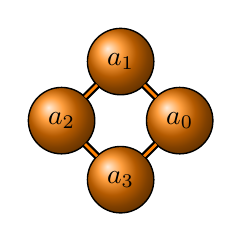
\begin{tikzpicture}[baseline=-0.65ex,scale=0.75]
      \SetVertexMath
      \GraphInit[vstyle=Shade]
      \grCycle[RA=1]{4}
    \end{tikzpicture}
    \qquad \Longrightarrow \qquad
    \begin{pmatrix}
      1 & 1 & 0 & 0 \\
      1 & 0 & 0 & 1 \\
      0 & 0 & 1 & 1 \\
      0 & 1 & 1 & 0 \\
    \end{pmatrix}
  \]

  Таким образом в каждой строке всегда будет по две единицы, по одной для каждого конца ребра.
  С такой матрицей решения COLUMN-COVER сможет решить и VERTEX-COVER, потому что для VERTEX-COVER нам нужно чтобы хотя бы один конец каждого ребра был включён во множество выбранных для покрытия вершин.
\end{document}
